\section{Datasets}
Throught the years,  there are so many excellent video segmentation datasets
\subsection{Datasets}

\paragraph{DAVIS}

Densely-Annotated VIdeo Segmentation is a  difficult challenge, which is mainly purposed for video object segmentation.
Frame resolution varies across sequences but all of them were downsampled to 480 p for the challenge. 
Pixel-wise annotations are provided for each frame for four different categories: human, animal, vehicle, and object.
DAVIS-2016 \cite{DAVIS2016}is composed by 50 high-definition sequences which add up to 2079 and 1376 frames for training and validation respectively.
This dataset mainly addresses problem on primary objects segmentaion, which means that there are at least one target foreground object in videos.
DAVIS-2017 \cite{DAVIS2017} have extended the number of sequences to 90, which is 60 sequences for training and 30 for validation, which contains 4209 and 1999 frames respectively.
They segment the main moving objects in the scene and divide them by their semantic, even though they might have the same motion. So we can refer DAVIS-2017 as the video instance segmentations.

\begin{figure}[ht]
    \centering
    \begin{subfigure}{}
        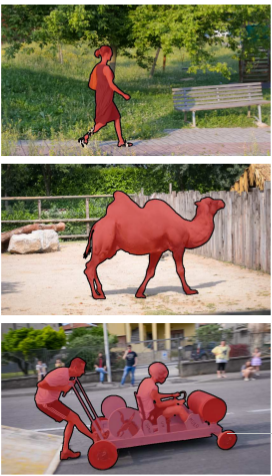
\includegraphics[width=0.2\textwidth]{figure/Davis_primary1.png}  
    \end{subfigure}
    \begin{subfigure}{}
        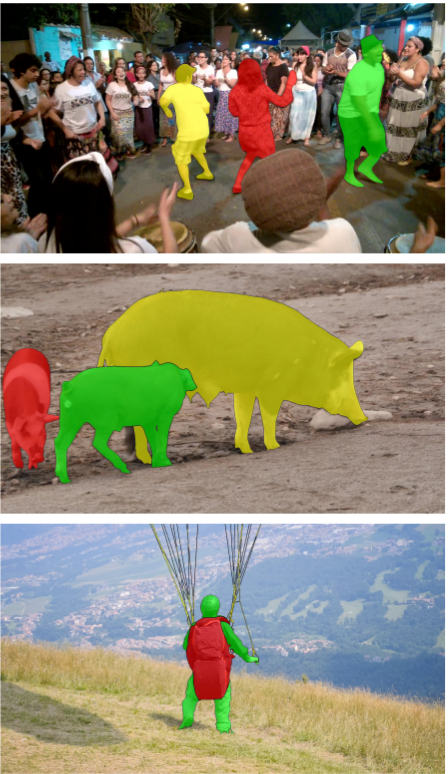
\includegraphics[width=0.2\textwidth]{figure/Davis_instance2.png}
    \end{subfigure}
    \caption{DAVIS dataset. The left is foreground segmentaion setting. The right is instance segmentation setting}
% 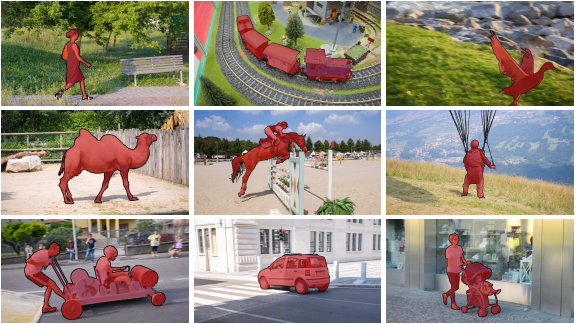
\includegraphics[width=0.45\textwidth]{figure/Davis_primary.png}    
\end{figure}


\paragraph{Youtube-Objects~\cite{Youtube}} 
The Youtube-Objects is a database of videos collected from YouTube which contain objects from ten PASCAL VOC classes: 
aeroplane, bird, boat, car,cat, cow, dog, horse, motorbike, and train.
That database does not contain pixel-wise annotations but Jain et al 
manually annotated a subset of 126 video sequences.
They took every 10th frame from those sequences and generated semantic labesl. 
That totals 10167 annotated frames at $480\times 360$ pixels resolution.

\paragraph{SegTrack-v2~\cite{SegTrack}}
The dataset is an updated version of the SegTrack dataset, which provide more additional
annotations of objects for other individual objects. The total 14 videos contain 1066 frames with pixel-
level annotations. 





